%!TEX root = ../main.tex
\subsubsection{Orthogonality and projection}
In this chapter we will explain the orthogonality in the context of Hilbert spaces and begin the discussion on projection on subspaces.

\paragraph{General definition} As we know from geometry, also in this context we can define orthogonality and orthonormality. In addiction, here we see how to characterize the Hilbert spaces.
\begin{defn}
	We say that $x$ and $y$ are \emph{orthogonal} if $$\sca{x,y} = 0;$$
	in such case we write $x \perp y$. \\
	Moreover, if $x \perp y$ and $\norm{x}=\norm{y}=1$, then we say that $x$ and $y$ are \emph{orthonormal}.
\end{defn}

\begin{prop}[Pythagoras' theorem]
	Let $x, y \in H$, $x, y \neq 0$.\\
	If $x \perp y$, then:
	$$\norm{x\pm y}^2 = \norm{x}^2 +\norm{y}^2.$$
\end{prop}
\begin{proof}
	Consider:
	$\norm{x+y}^2 = \norm{x}^2 + 2\sca{x,y} + \norm{y}^2 = \norm{x}^2 +\norm{y}^2$.\\
	Same in the case of minus.
\end{proof}

\paragraph{Extending to set} This notion can be extended from points to sets:
\begin{defn}
	Let $(H, \sca{\cdot, \cdot})$ be a Hilbert space, and $V \subset H$.\\
	Then we define the \emph{orthogonal set} of $V$ as follows: 
	$$V^\perp \coloneqq \{x \in H : \ \sca{x,v}=0, \ \forall v \in V\}.$$
\end{defn}

\begin{prop}
	The set $V^\perp$ is always a closed subspace of $V$.\\
	Moreover, we have:
	$$ \widebar{V}^\perp = V^\perp \text{ and } \widebar{(\text{span}V)}^\perp = V^\perp.$$
\end{prop}
The proof is easy and left as an exercise to the reader.

\begin{defn}
	Let $(H, \sca{\cdot, \cdot})$ be a Hilbert space, and $V,W \subset H$ be subspaces.\\
	We say that $V$ and $W$ are \emph{orthogonal subspaces}, and we write $V \perp W$, if:
	$$V = W^\perp \text{ and } W = V^\perp$$
	that means:
	$$v \perp w \quad \forall v \in V, w \in W.$$
	In this case we set the subspace \emph{direct sum} of $V$ and $W$ as follows:
	$$ V \oplus W \coloneqq \{v+w : v \in V, w \in W \}.$$ 
\end{defn}

\begin{prop}
	If $V \perp W$, then $V \cap W=\{0\}$,
	and any element $x \in V \oplus W$ has a unique representation as $v+w$.
\end{prop}

\paragraph{Projections} These definitions concludes our introduction to orthogonality. Now we see this notion in action.

\begin{theo}[projection theorem]\label{theo-projection}
	Let $(H, \sca{\cdot, \cdot})$ be a Hilbert space, and $V \subset H$ be a closed subspace.\\
	Then we can write $H$ as:
	$$H= V \oplus V^\perp.$$
	This is also called \emph{orthogonal decomposition} of $H$.
\end{theo}

Observe that, on account of this theorem, if $V$ is a subspace of $H$, then: 
$$( V^\perp )^\perp = \widebar V.$$
Indeed, we have:
\begin{align*}
	V^\perp \ \text{closed} &\implies H = V^\perp \oplus ( V^\perp )^\perp = ( V^\perp )^\perp \oplus V^\perp,\\
	\widebar V \ \text{closed} &\implies H = \widebar V \oplus ( \widebar V )^\perp = \widebar V \oplus V^\perp.
\end{align*}

Note also that $V^\perp =\{0\}$ if and only if $\widebar V = H$.\\
This is because $V^\perp = \{0\}$ so that $(V^\perp)^\perp = H$ and $\widebar V = H$.\\
Viceversa, from $\widebar V = H$ we find $V ^\perp = ( V^\perp )^\perp = \{0\}$. To sum up, we say that $V$ is dense in $H$ if and only if $V^\perp = \{0\}$.

\begin{proof}
	Let $x \in H$. Due to minimal distance theorem \vref{theo-min-dist}, supposing $V$ non-empty, there exists a unique $v \in V$ such that $d(x,V) = \norm{x-v}$.
	
	Set now $w \coloneqq x - v$ and choose $\lambda \neq 0$ such that for any $u \in V$ we have $\lambda \sca{w, u} \geq 0$.
	\begin{figure}[htpb]
		\centering
		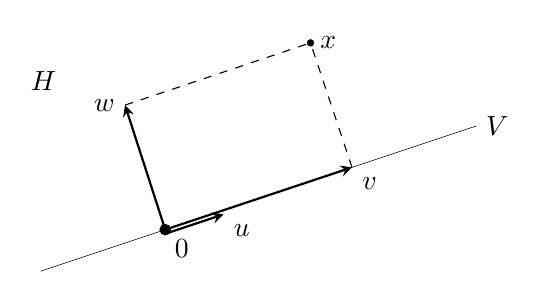
\begin{tikzpicture}[x=0.75pt,y=0.75pt,yscale=-1,xscale=1]
		\coordinate[label=below right:$0$] (O) at (200,190);

		\draw [very thin] (140,210) -- (350,140) node [right] {$V$};
		\draw (134,112.4) node [anchor=north west][inner sep=0.75pt] {$H$};

		\draw [fill=black] (O) circle (2.5);

		\draw [thick, -stealth] (O) -- (180.63,130) node [left] {$w$};
		\draw [thick, -stealth] (200,192) -- (228.1,182.63) node [below right] {$u$};
		\draw [thick, -stealth] (O) -- (290,160) node [below right] {$v$};

		\draw[fill=black] (270,100) circle (1.5) node[right] {$x$};
		\draw [dashed, thin] (290,160) -- (270,100);
		\draw [dashed, thin] (180.63,130) -- (270,100);
		\end{tikzpicture}
		\caption{Geometric intuition behind the proof of the projection theorem.}
	\end{figure}
	\FloatBarrier
	Then we have:
	\begin{align*}
		\inf_{y \in V} \norm{x-y}^2 &= \norm{w}^2\\
		&\leq \norm{x-\underbrace{(v+\lambda u)}_{\in V}}^2\\
		&= \norm{w- \lambda u}^2\\
		& = \norm{w}^2-2\lambda\sca{w,u} + \lambda^2 \norm{u}^2.
	\end{align*}
	Then we have $-2 \lambda \sca{w, u} + \lambda^2 \norm{u}^2 \geq 0$, thus $\lambda^2 \norm{u}^2 \geq 2 \lambda \sca{w,n}$ which implies 
	$$
		|\sca{w, u}| < \frac{|\lambda|}{2}\norm{u}^2.
	$$
	Letting $\lambda$ go to zero, we get:
	$$\sca{w,n} = 0 \quad \forall u \in V.$$
	Thus we have proven that $x=v+w$ where $w\in W=V^{\perp}$.\\
	We are left to prove that $V=W^{\perp}$ so that $H=V\oplus V^{\perp}$.\\
	Observe that $V\subset W^{\perp}$.\\
	On the other hand if $x\in W^{\perp}$ then:
	$$
		x=u^{\star} +w^{\star} ,\ \ u^{\star} \in V,w^{\star} \in W.
	$$
	Thus $x-u^{\star} \in W\cap W^{\perp} =\{0\}$ and this gives $x=u^{\star}$ so that $x\in V$.
\end{proof}
On account of this theorem we can give the following definition.

\begin{defn}[orthogonal projectors]
	Let $(H, \sca{\cdot, \cdot})$ be a Hilbert space, and $V \subset H$ be a closed subspace.\\
	Let also $v$ the unique element of $V$ such that $\norm{x-v} = d(x, V)$.\\
	Define the following \emph{projector} of $H$ onto $V$:
	$$P_V : H \to V  \quad P_V x = v.$$
	In the same way we can define the projector of $H$ onto $V^\perp$:
	$$P_{V^\perp}: H \to V^\perp \quad P_{V^\perp} x = x-v = x - P_V x.$$
\end{defn}
Notice that $x = P_V x + P_{V^\perp} x$.

$P_V$ is linear and bounded, namely: $$P_V \in \Bc(H, H).$$

\begin{itemize}
\item boundedness is easy:
$$
	\norm{x}^2 =\Vert P_V x\Vert^2 +\norm{P_{V^{\perp}} x}^2 \ \ \implies  \ \ \norm{P_V x} \leq \norm{x} 
$$
\item linearity is a bit harder:
$$
	\begin{drcases}
	\alpha x-P_V( \alpha x) \in V^{\perp}\\
	\alpha x-\alpha P_V(x) \in V^{\perp}
	\end{drcases}
	\implies \cancel{\alpha x}-P_V( \alpha x) -[\cancel{\alpha x} -\alpha P_V(x)] \in V^{\perp}
$$
but also
$$
	\alpha \underbrace{P_V(x)}_{\in V} -\underbrace{P_V( \alpha x)}_{\in V} \in V
$$
thus
$$
	\alpha P_V(x) -P_V( \alpha x) \in V^{\perp} \cap V=\{0\} \ \ \implies  \ \ \alpha P_V(x) =P_V( \alpha x)
$$
A similar argument can be done to prove that $P_V(x) +P_V(y) =P_V(x+y)$.
\end{itemize}

%\begin{rema} % Possible repetition?
%	Let $(H, \sca{\cdot, \cdot})$ be a Hilbert space, and $V \subset H$ be a closed subspace. \\
%	Then $(V^\perp)^\perp = V$, and $V^\perp = \{0\}$ if and only if $V=H$. \\
%	Notice that, if $V$ is not closed, $V^\perp = \{0\}$ if and only if $\widebar V = H$.
%\end{rema}
